


\section{Evaluation}
\label{sec:evaluation}

This section describes our experimental setting and evaluation method to compare Augmented BO with Naive BO.
\subsection{Experimental Method}
\label{sec:experiment}

\subsubsection*{Workload}
For evaluation, we use Apache Hadoop (v2.7) and Spark (v2.1 and v1.5).
We choose distinct workloads from \emph{HiBench} and \emph{spark-perf}, as listed in \mytable{\ref{tab:dataset}}.
\emph{HiBench} is a big data benchmark suite for Apache Hadoop and Spark \cite{hibench}.
It was designed to test batch processing jobs and streaming workloads. Similarly, \emph{spark-perf} is a performance testing suite for Spark \cite{sparkperf}.
The testing suite provides a wide range of workloads including
supervised learning such as regression and classification modeling,
unsupervised learning such as K-Means clustering,
and statistical tools such as correlation analysis, and Principal Component Analysis (PCA).
We run 107 workloads to test their performance on 18 VM types.
During the execution of the workload, a \emph{sysstat} demon is run in the background to collect low-level performance information~\cite{sysstat}.
There is no observable overhead to this data collection.



\subsubsection*{Cloud Configurations}
We measure the performance on six VM families (available on AWS)
\{\emph{c3}, \emph{c4}, \emph{m3}, \emph{m4}, \emph{r3} and \emph{r4}\}, and
three VM sizes \{\emph{large}, \emph{xlarge} and \emph{2xlarge}\}.\footnote{The latest generation has been upgraded
from \emph{c4} to \emph{c5} for the compute-optimized VM and from \emph{m4} to \emph{m5} for the general-purpose VM
after we completed our data collection.}
The VM size represents the core count.
For example, \emph{c4.large} has two cores,
\emph{c4.xlarge} has four cores and \emph{c4.2xlarge} has eight cores. 

\subsubsection*{Encode Cloud Configurations}
Each VM type is characterized by CPU types, core count, average RAM per core, and the bandwidth to Elastic Block Storage (EBS). We encode the four features with numerical values into $\vec{\mathit{VM}}$. The CPU types are encoded from one to six in order, and for the core count, we use their actual values \{2, 4, 8\}.
Similarly, the RAM size per core is \{2, 4, 8\} GB. Last, the bandwidth to EBS has three classes for different VM types encoded as \{1, 2, 3\}.

% 
% \noindent {\textit{Implementations}}:
% We implement naive BO as described in \emph{CherryPick}~\cite{Alipourfard2017}.
% Our proposed method is low-level augmented Bayesian Optimization (Augmented BO). Our goal is to test whether Augmented BO can find the best VM for a workload and compare its search cost to naive BO.

\begin{figure}[!htbp]
\centering
\begin{subfigure}[b]{0.8\textwidth}
    \centering
    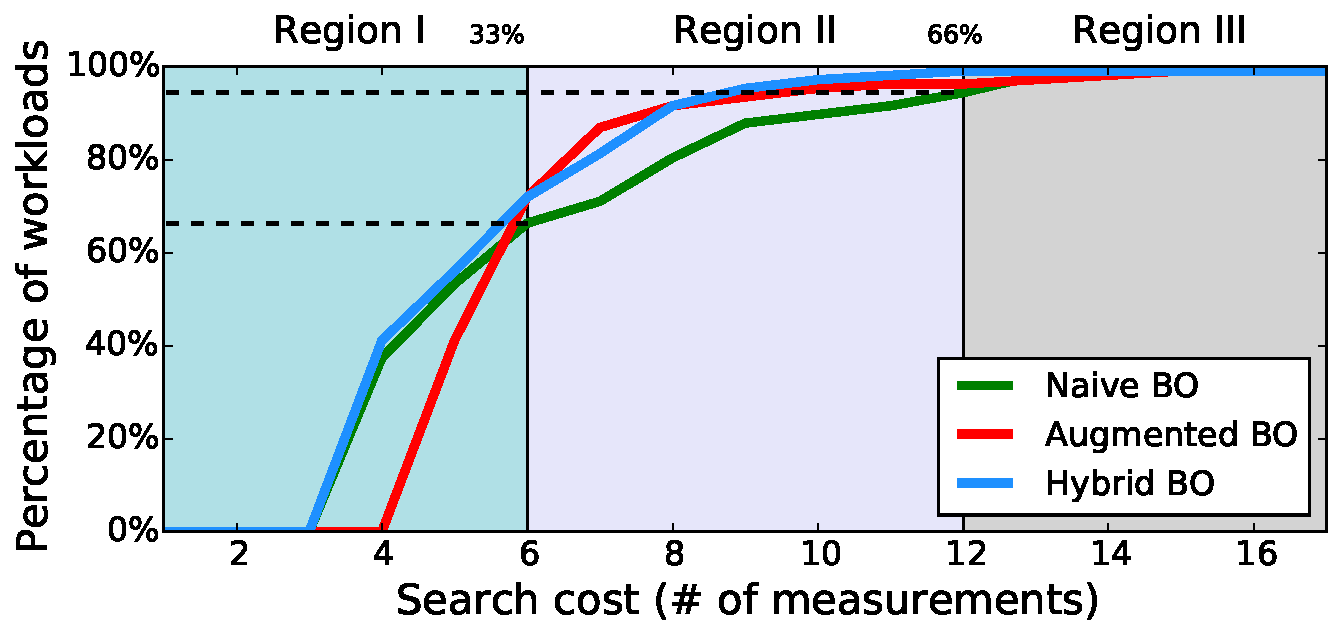
\includegraphics[width=\linewidth]{figures/overall_time_new.pdf}
    \caption{Optimizing running time}
    \label{fig:overall_time}
\end{subfigure}
\begin{subfigure}[b]{0.8\textwidth}
    \centering
    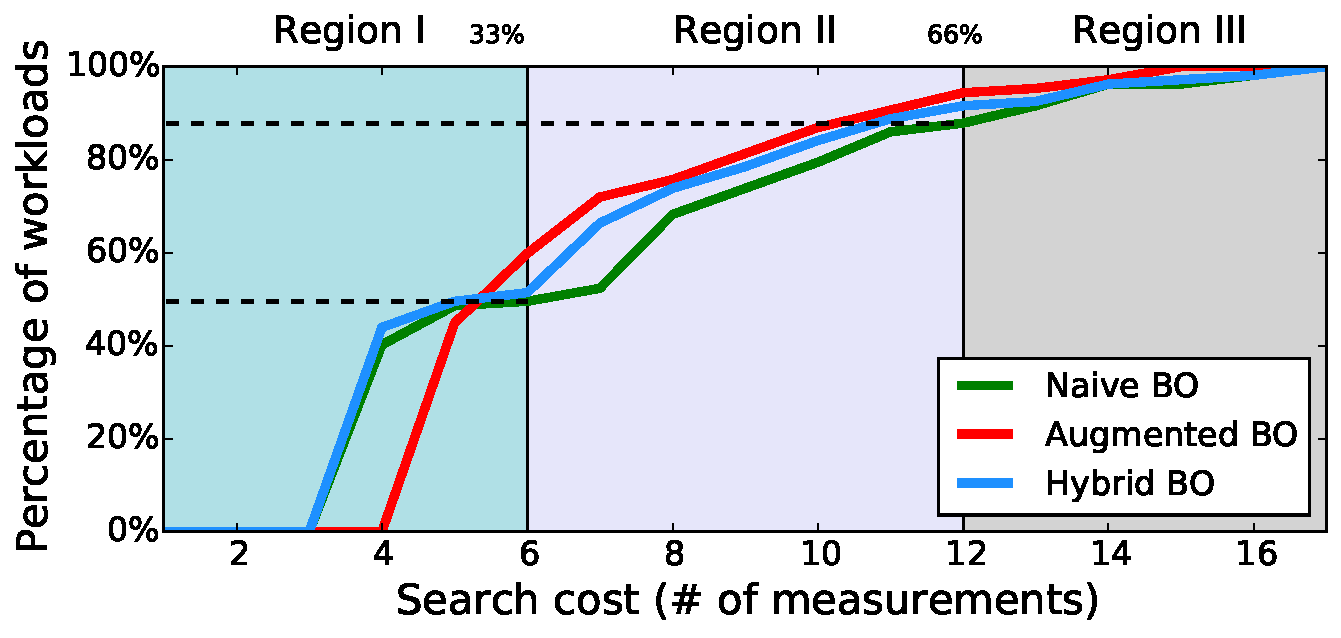
\includegraphics[width=\linewidth]{figures/overall_cost_new.pdf}
    \caption{Optimizing running cost}
    \label{fig:overall_cost}
\end{subfigure}
\caption{Search cost of finding the optimal VM type across the 107 workloads. The \emph{y-axis} represents the cumulative percentages of workloads.
 In \emph{Region I}, although Augmented BO does not find the optimal VM type at the fourth step, it does find a very near optimal solution with only 4\% difference.
 Section~\ref{sec:practice} provides further details.}
\label{fig:overall}
\end{figure}

\subsection{Comparison}
\label{sec:comparison}
This section evaluates Naive BO and Augmented BO on the 107 workloads with randomly selected initial VMs. The above process is repeated 100 times to account for variance.
Here we minimize execution time and deployment cost individually. 
\myfigure{\ref{fig:overall}} presents the overall result. %\textit{Please note that Figure~\ref{fig:overall} only reports the performance of a method to find the optimal VM}. 



\subsubsection*{Can Augmented BO find optimal VMs?}

Figure~\ref{fig:overall_time} shows the percentage of workloads, where Naive BO and Augmented BO find the optimal VM.
The horizontal axis represents the search cost (in terms of the number of measurements), and the vertical axis represents the percentage of the workloads. In this figure the \textcolor{green}{green} line represent the Naive BO and the \textcolor{red}{red} line represent the Augmented BO. The Naive BO can find the optimal solution for 60\% of the workloads by searching 33\% of the search space (Region I). The performance of Augmented BO is similar to naive BO. However, Augmented BO has a slow start problem but becomes effective eventually. In Region II, Augmented BO is a clear winner as it can find optimal VMs for 96\% of the workloads within ten measurements. At the same time, Naive BO can only find 80\% of the workload.

We claim that the performance of Augmented BO is better than Naive BO, for regions I and II (at step 6 and 12). We also observe an interesting phenomenon---Augmented BO is outperformed by Naive BO in initial four steps. The one-step difference can be attributed to the over-fitting problem caused by
the larger training features (both high-level and low-level information) in Augmented BO. This is a challenge of leveraging low-level information (for future work). 

While looking at the performance of VMs selected by Augmented BO, we observe that the best VM found by Augmented BO is only 4\% away from the optimal VM. In practice, this difference can be easily ignored (refer to
Section~\ref{sec:practice}). Furthermore, with the growing instance space,
this difference (though we believe is little) can be amortized because
the search cost will also increase.

A possible workaround to this problem can be to create a Hybrid BO (shown in \textcolor{blue}{blue})---which combines the best of the two methods.
\myfigure{\ref{fig:overall_time}} shows that \emph{Hybrid BO}
outperforms Naive BO in all cases.
However, we choose not to focus on the hybrid method here
because our primary objective is to identify the fragility of Naive BO and the advantages of leveraging low-level information.
Please refer to Section~\ref{sec:arrow::hybrid} in more detail.


\subsubsection*{Can Augmented BO minimize cost?}

To answer the question if Augmented BO can minimize the deployment cost, it is essential to demonstrate that Augmented BO can find optimal VM faster than Naive BO (lower search cost). In Figure~\ref{fig:overall_cost}, we observe that \textit{minimizing deployment cost is more difficult} than minimizing execution time, \ie{both methods require more search cost to reach the optimal solution}.
Naive BO can find the best VM with six attempts
for only 50\% applications while Augmented BO increases this probability to 60\%. We also see a clear win for Augmented BO as it can find best VM which minimizes the deployment cost after measuring five measurements. However, we see that Augmented suffers from a slow start, which is similar to Figure~\ref{fig:overall_time} and  Hybrid BO (shown in \textcolor{blue}{blue}) is the workaround. 


\subsubsection*{Is Augmented BO fragile?}

In finding the best VM, Naive BO fails
in 36\% (minimizing time) and 50\% (minimizing cost) of the workloads
after measuring the performance of the six VMs (Region I).
Augmented BO alleviates this problem, and this can be observed by a
up to 20\% increase in the number of workloads for which Augment BO found the optimal VM (step 7 in~\myfigure{\ref{fig:overall_cost}}).

Stability is another important aspect of Augmented BO. As discussed in Section~\ref{sec:init_points},
initial points are critical to the performance of BO---different initial VMs can lead to very different results (performance and search cost) or high variances in results. \myfigure{\ref{fig:convergence_time}} compares the search cost and the performance found by the two methods. We present the median value (shown by line), and the interquartile range (the difference between the $3^{rd}$ and the $1^{st}$ quartile) shown by the shaded region. The three cases show that Augmented BO yields less search cost and reduces the variance. This demonstrates  Augmented BO is not fragile.

Another interesting observation is that
Augmented BO not only alleviates the fragile problem in \emph{Region II} but also
moves workloads from \emph{Region III} to \emph{Region II}.
~\myfigure{\ref{fig:convergence_time_1}} and
~\myfigure{\ref{fig:convergence_time_2}} are example workloads
in \emph{Region III} for Naive BO.
The first quartile indicates that Augmented BO finds the optimal configuration
even with four or five attempts in 25\% initial points that are tested.




\begin{figure}[!htbp]
\centering
\begin{subfigure}[t]{0.6\textwidth}
    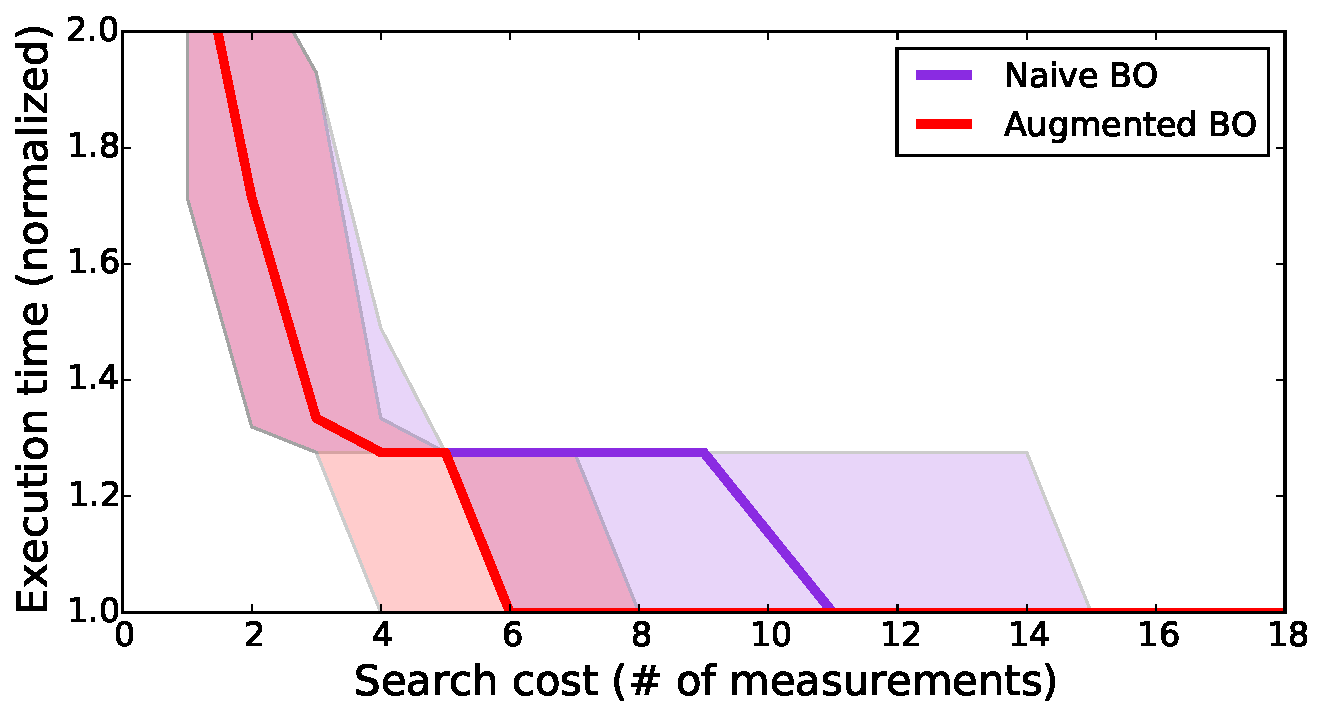
\includegraphics[width=\linewidth]{figures/time_hadoop.pagerank.large.pdf}
    \caption{PageRank on Hadoop 2.7}
    \label{fig:convergence_time_1}
\end{subfigure}
\begin{subfigure}[t]{0.6\textwidth}
    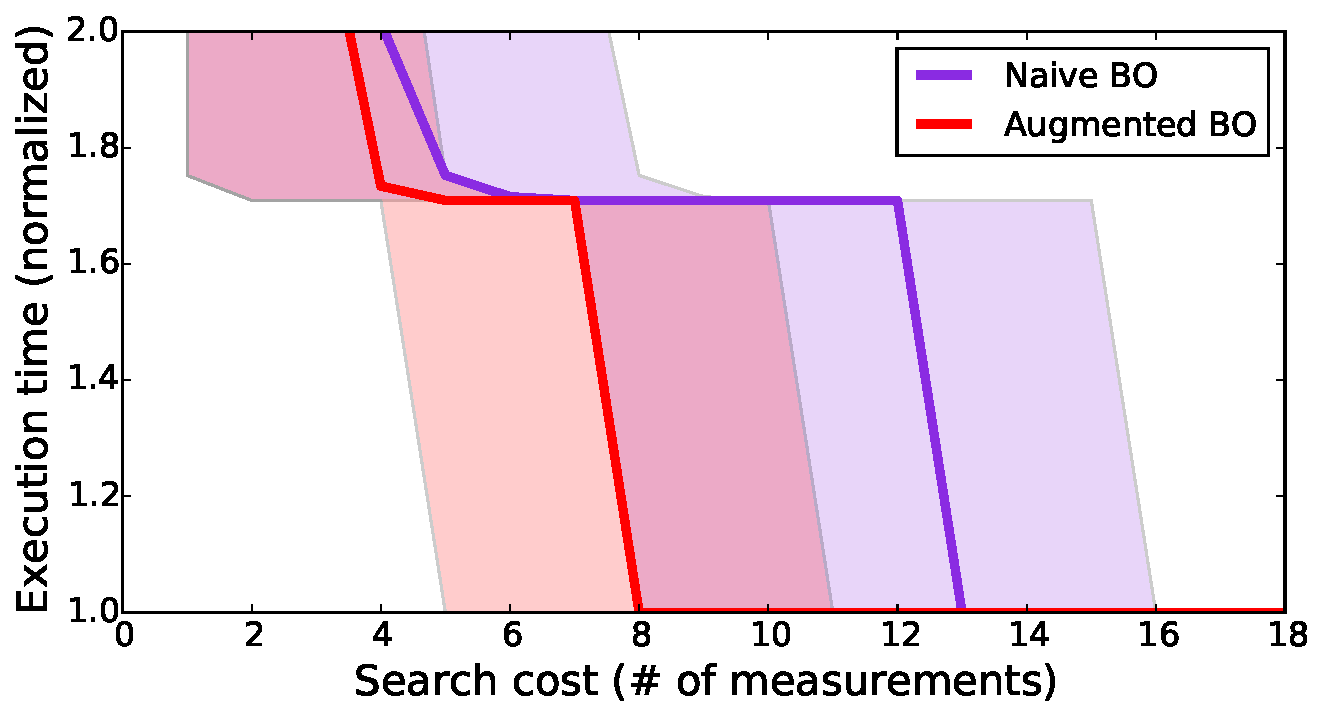
\includegraphics[width=\linewidth]{figures/time_spark.als.large.pdf}
    \caption{Alternating Least Squares on Spark 2.1}
    \label{fig:convergence_time_2}
\end{subfigure}
\begin{subfigure}[t]{0.6\textwidth}
    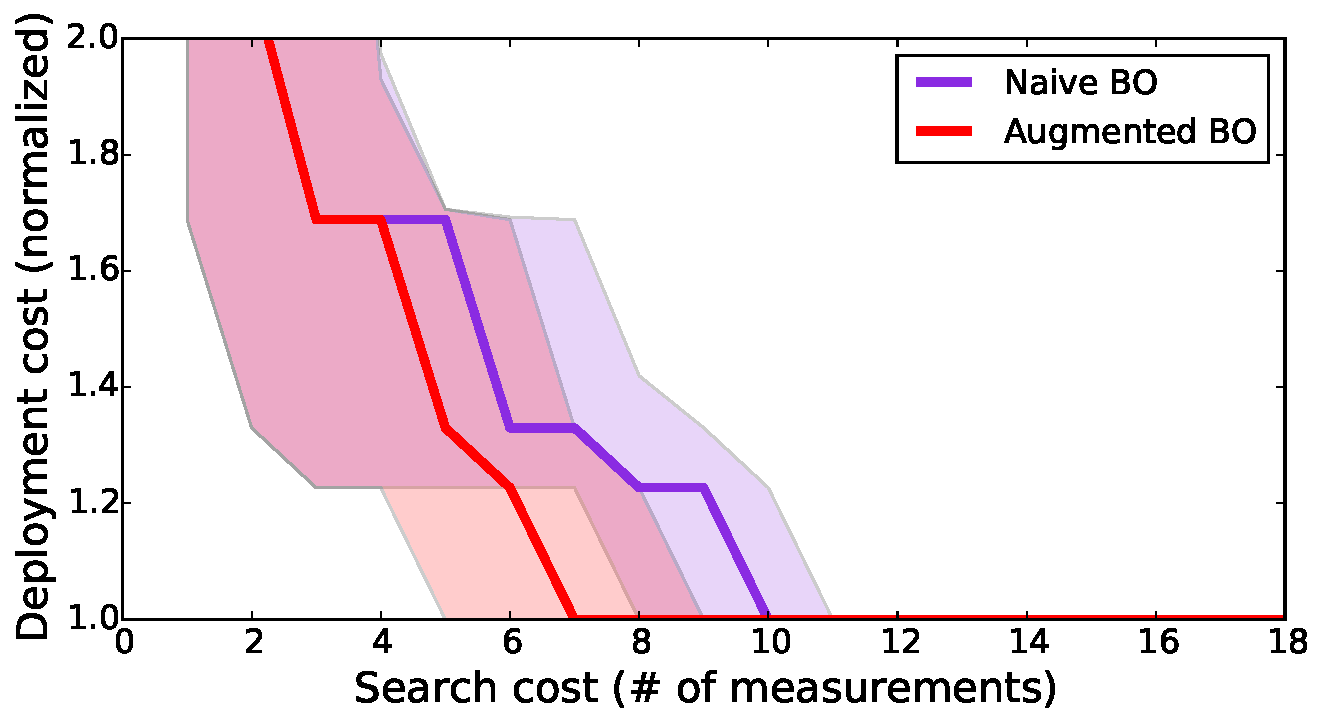
\includegraphics[width=\linewidth]{figures/cost_spark.lr.small.pdf}
    \caption{Logistic Regression on Spark 1.5}
    \label{fig:convergence_cost_2}
\end{subfigure}
\caption{
Examples of searching for the best VM. The objective is to find the fastest VM in subfigures (a, b) and the most cost-effective VM in subfigure (c).  Both the BO methods stops after they find the optimal VM type (normalized to 1.0).  The line represents the median value of the execution time over 100 repeats. Each repeat used different initial points to seed BO. The shaded region represents the IQR or Interquartile range is the difference between $3^{rd}$ and $1^{st}$ quartile. A high value (larger area) of IQR indicates high variance.}
\label{fig:convergence_time}
\end{figure}



\section{Discussion}
\label{sec:practice}

\subsection{Bayesian Optimization in Practice}
\label{sec:bo_practise}
In practice, users can tolerate a loss in performance (deployment cost or execution time) in exchange for lower search cost. In this section, we examine the performance of the two methods
when we (slightly) relax the definition of optimality.
% we (slightly) relax the performance objective from optimal VM to near optimal VM.
Due to space limitations, we only present the results of minimizing deployment cost as we have shown it is more challenging, and the conclusion is similar to minimizing execution time.

To demonstrate the performance (of BO) and search cost trade-off, we vary the stopping criteria to understand how they affect both search cost and the best VM they find. 
% Stopping criteria can either be defined in terms of the number of measurements or the predicted improvement (in the estimated performance).
We choose EI as the stopping criteria for Naive BO (as prescribed by \emph{CherryPick}). For Augmented BO, we use Prediction Delta and vary the thresholds from 0.9 to 1.3. We examine the three regions separately to analyze the effects of stopping criterion on different categories of workload.

% In Figure~\ref{fig:convergence_cost} presents the results. The horizontal axis represents the search cost, and the vertical axis represents the performance (\textcolor{red}{which one?}).
In Figure~\ref{fig:stopping_criteria_comparison_good}, Naive BO finds the optimal VM regardless of the stopping criteria. This is counter-intuitive because there should exist a trade-off between the deployment cost and the search cost. We hypothesize that Naive BO cannot estimate that it has found the optimal VM. Augmented BO, on the other hand, clearly shows the trade-off. Augmented BO with the thresholds $1.25$ and $1.3$ performs similarly to Naive BO.
%As pragmatic engineers, we are always hard-pressed to recommend Naive BO over Augmented BO, which achieves a performance of 1.04 rather than a perfect 1.0. 

In Figures~\ref{fig:stopping_criteria_comparison_bad} and~\ref{fig:stopping_criteria_comparison_problematic}, Augmented BO is the clear winner. With the $1.1$ threshold, Augmented BO outperforms Naive BO in both
the search cost and the deployment cost. To simplify the comparison, we choose 10\% EI for Naive BO (as prescribed by \emph{CherryPick}) and 1.1 threshold for Augmented BO. Our method yields lower search cost while achieving lower deployment cost. On average, it finds VMs with 5\% lower in deployment cost while reducing search cost by 20\%.
This demonstrates that the low-level augmented Bayesian Optimization finds the well-suited VMs quicker and is more precise when compared to Naive BO.

Overall, we recommend using $1.1$ threshold in Augmented BO since
the deployment cost is comparable with Naive BO and reduces
the search cost.
In \myfigure{\ref{fig:comparison_cost}},
we present the overall comparison of the two methods with the EI and threshold
described above. The horizontal axis represents the reduction in search cost, and the vertical axis represents the decrease in the deployment cost (higher the better in both).
% \footnote{We compare the deployment cost because (i) space restrictions and (ii) optimizing for deployment cost is harder than optimizing for running time.}
The figure shows the result for all 107 workloads represented as points. Points enclosed with lines $x \geq 0$ and $y \geq 0$ (shown in \textcolor{blue}{blue} shade) indicates workloads, where Augmented BO can find VMs with lower deployment cost and lower search cost. For example, the workload represented in (24, 10) is the case where Augmented BO uses 24\% lower search cost, and the best VM found (for that workload) has 10\% lower deployment cost than the one found by Naive BO. There are 46 such workloads.
Augmented BO requires higher search cost than Naive BO in five workloads (region shaded in \textcolor{red}{red}). But they both find the optimal solution.
There are 17 workloads where Augmented BO finds VM types with higher running cost
but with lower search cost---a region of trade-off.


\begin{figure}[!htbp]
\centering
\begin{subfigure}[b]{0.5\textwidth}
    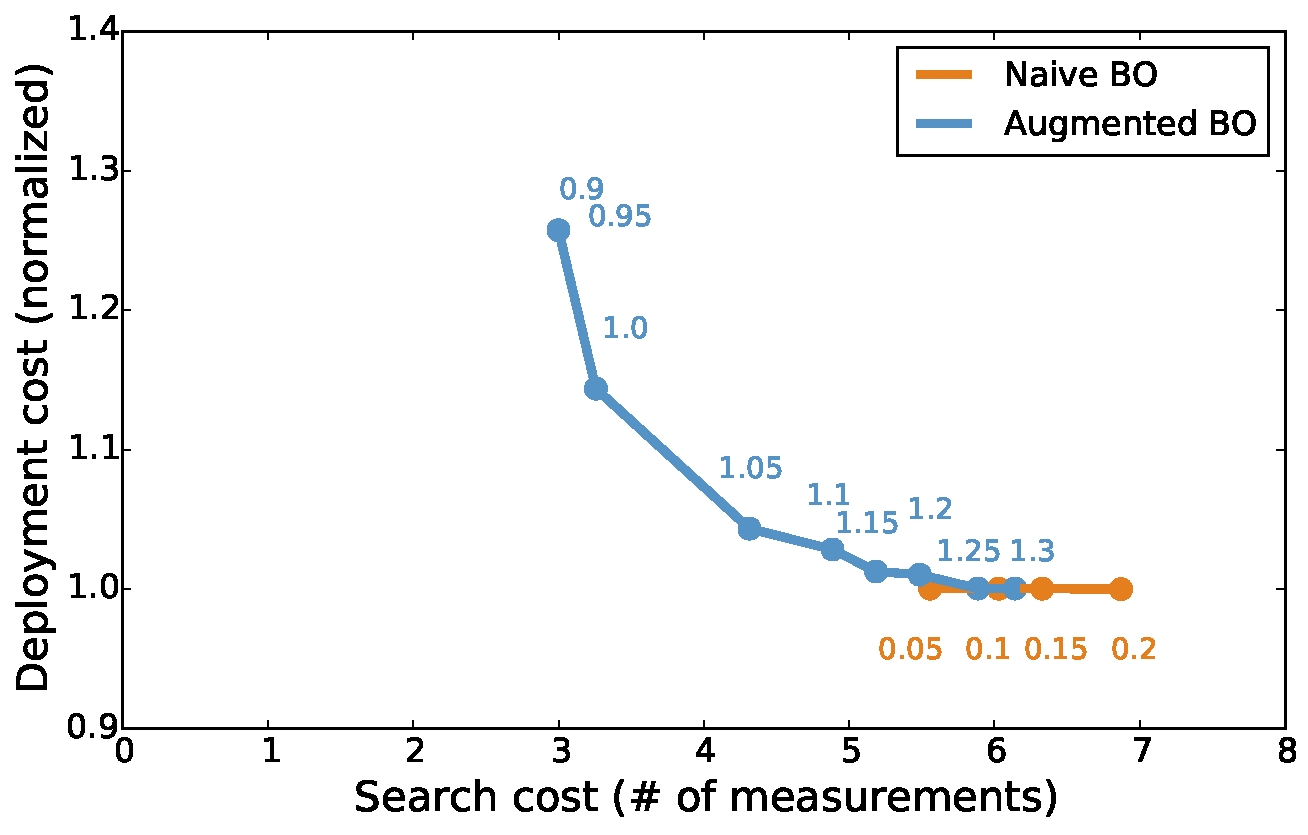
\includegraphics[width=\linewidth]{figures/stopping_criteria_comparison_cost_good.pdf}
    \caption{Region I}
    \label{fig:stopping_criteria_comparison_good}
\end{subfigure}
\begin{subfigure}[b]{0.5\textwidth}
    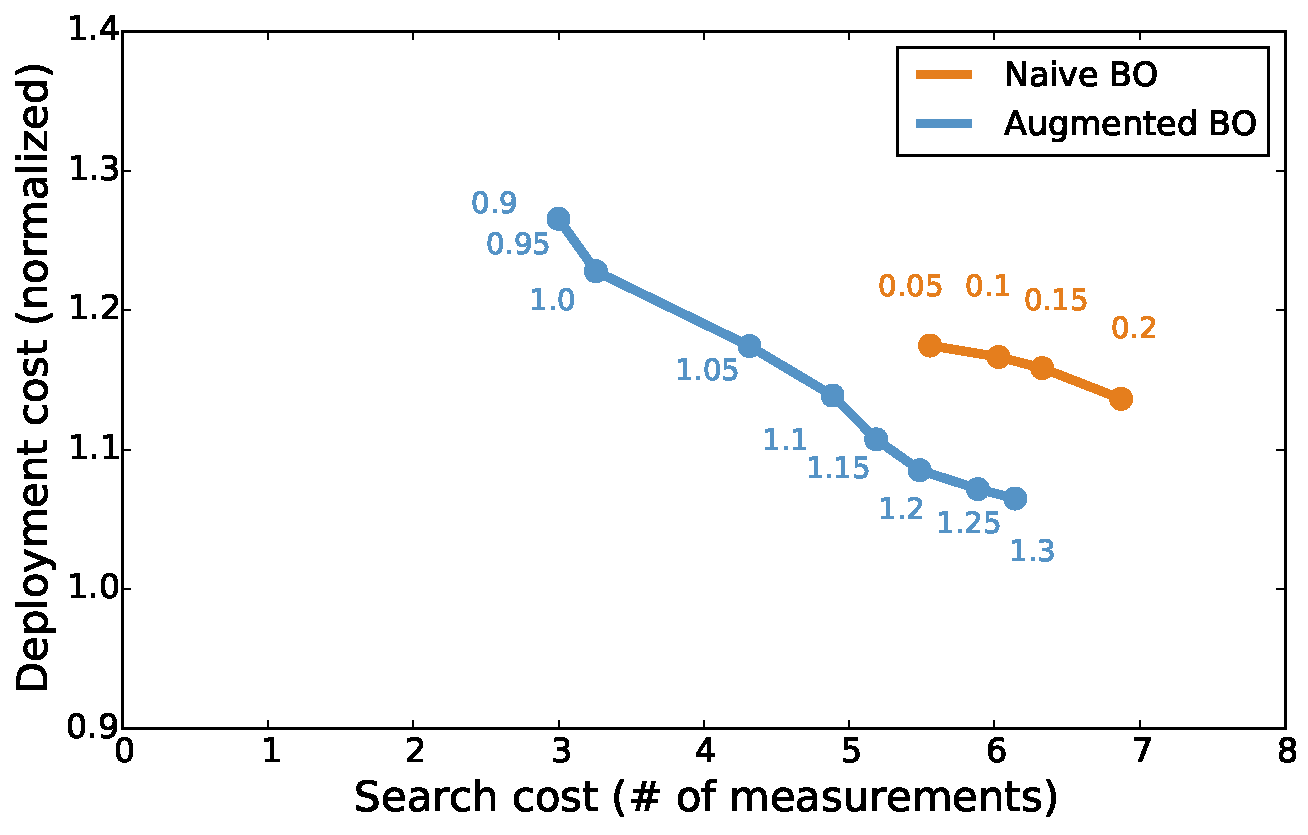
\includegraphics[width=\linewidth]{figures/stopping_criteria_comparison_cost_bad.pdf}
    \caption{Region II}
    \label{fig:stopping_criteria_comparison_bad}
\end{subfigure}
\begin{subfigure}[b]{0.5\textwidth}
    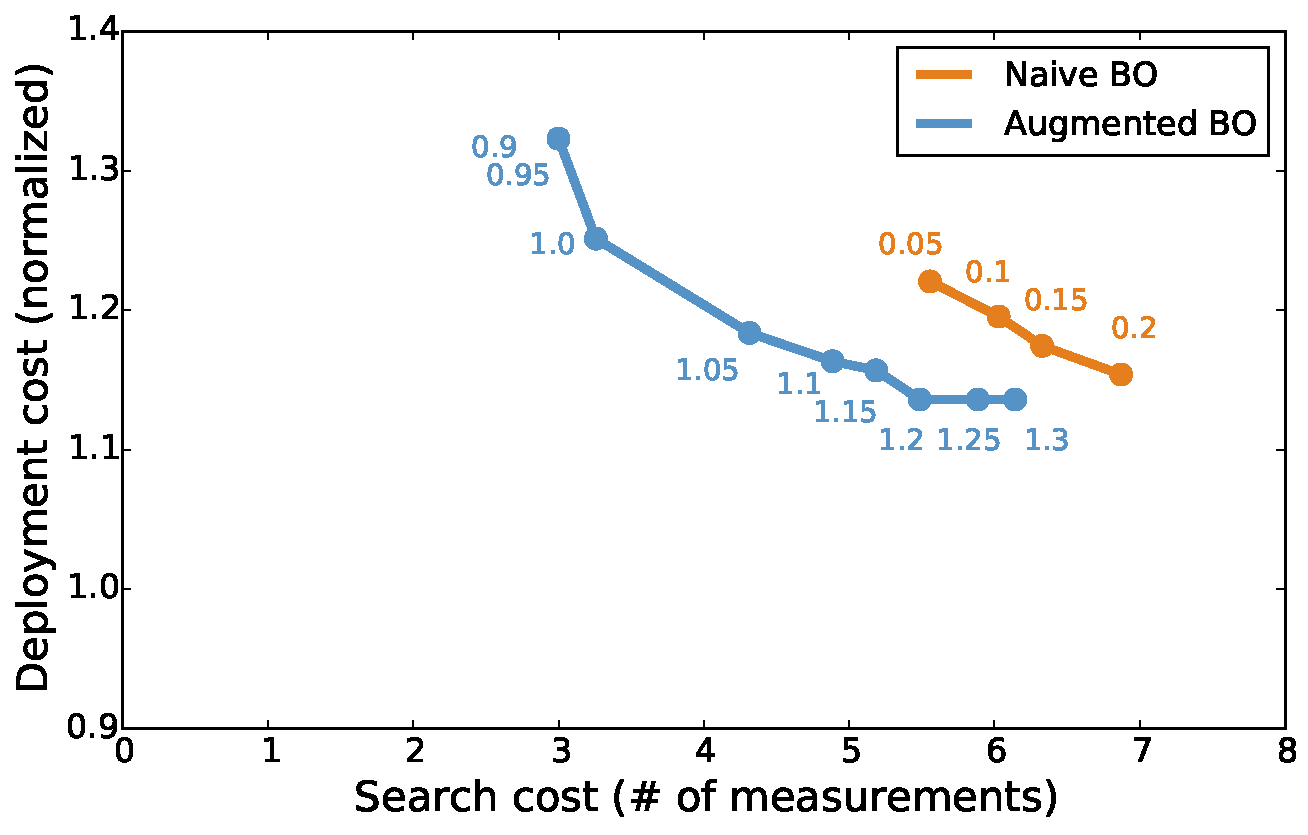
\includegraphics[width=\linewidth]{figures/stopping_criteria_comparison_cost_problematic.pdf}
    \caption{Region III}
    \label{fig:stopping_criteria_comparison_problematic}
\end{subfigure}
\caption{Comparison between effectiveness of search with different stopping criteria.  There is a trade-off between search cost and deployment cost. In \emph{Region I}, Augmented BO is comparable with Naive BO in terms of deployment cost but can greatly reduce search cost at the expense of slight increase in deploymwnr cost. For \emph{Region II} and \emph{Region III}, Augmented BO outperform Naive BO for both search cost and deployment cost.}
\label{fig:stopping_criteria_comparison}
\end{figure}


\subsection{Time-Cost Trade-off}
\label{sec:tradeoff}

This section demonstrates how to adapt Augmented BO as well as Naive BO to navigate the time-cost trade-off. In practice, a user would always want a solution to reduce time as well as cost. We propose a new measure called time-cost product which is similar to an energy-time trade-off in high-performance computing~\cite{Freeh2007}.
% cloud computing exhibits a trade-off between execution time and deployment cost
Not every time-cost trade-off is desirable because
a small improvement in performance may incur a higher running cost.
For example, a 10\% improvement in execution time requires
a 50\% increase in deployment cost. 
% We examine the support of Augmented BO on the Performance-Search Cost trade-off.

For simplicity, we assign the same importance to time and cost.
That is, it is considered desirable for a 10\% improvement in time and
a 10\% increase in cost.
To support the time-cost trade-off, instead of predicting the execution time
and deployment cost, the surrogate model estimates the product of time and cost. Any two VMs are considered the same if their products of execution time and deployment cost are the same.
Similarly, a larger product represents an undesirable choice.

\myfigure{\ref{fig:comparison_cdp_1.05}}  presents the comparison which is similar to Figure~\ref{fig:comparison_cost}. We observe a great reduction, \ie{$>50\%$} in search cost.
Naive BO exhibits long searching process (more than six attempts) in 24\% of the 107 workloads and very long searching (at least ten attempts) in 13\% workloads. On the other hand, Augmented BO requires no more than 6 actual evaluation
for all 107 applications. Please note that the threshold used for this experiment is 1.05, which also tells us that the stopping criteria also need to be changed based on the workload as well as the performance objective.

\begin{figure}[!htbp]
    \centering
    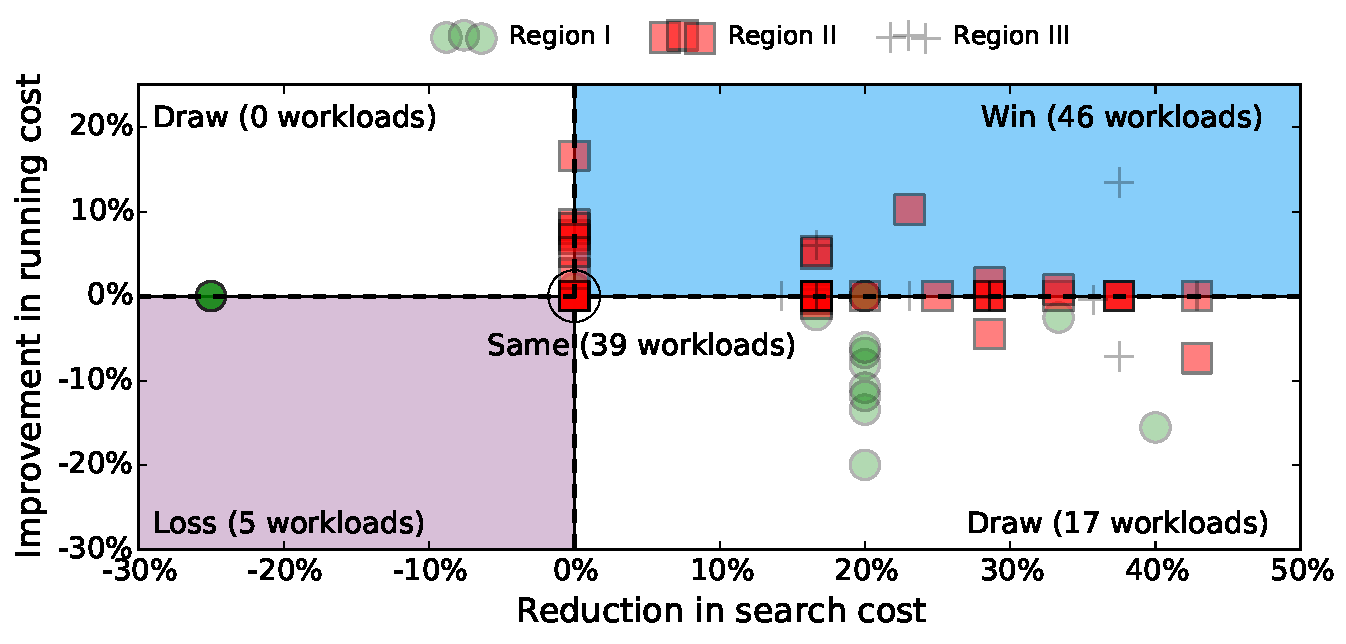
\includegraphics[width=0.8\textwidth]{figures/comparison_cost.pdf}
    \caption{Overall comparison for the two BO methods in finding the most cost-effective VM type across the evaluated 107 workloads. The numbers are calculated as the reduction percentage in search cost and improvement in deployment cost, both higher the better. Workloads in (0,0) represent workload which achieve similar performance in both methods.}
    \label{fig:comparison_cost}
\end{figure}

\begin{figure}[!htbp]
    \centering
    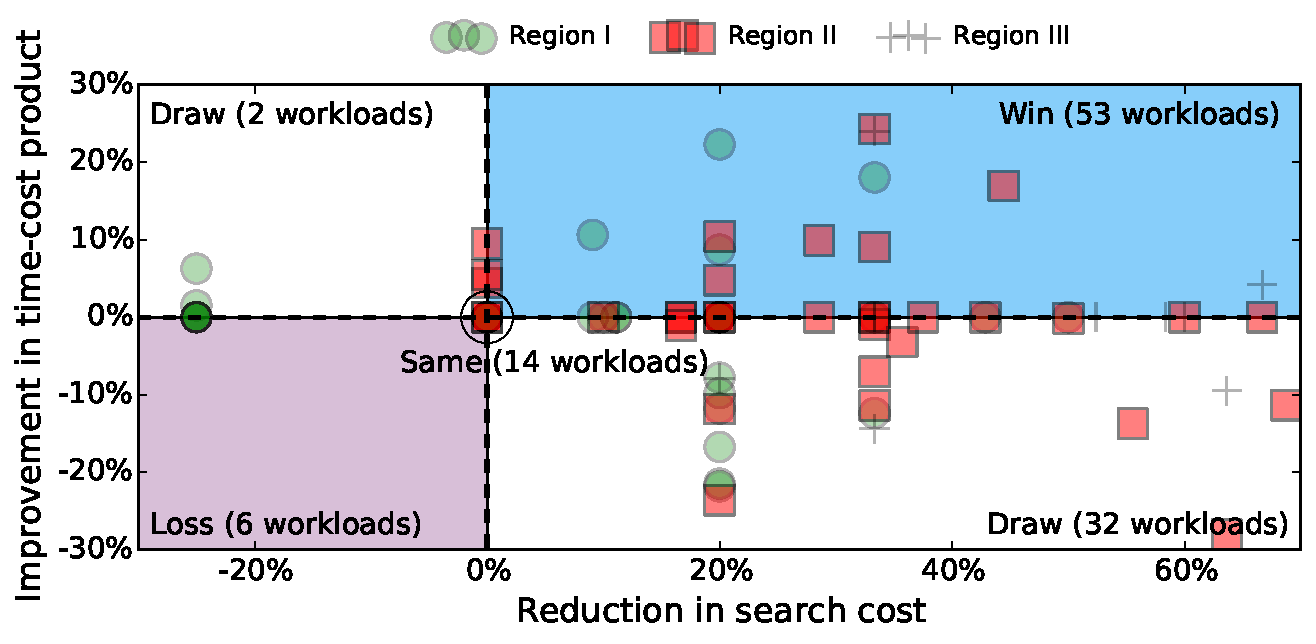
\includegraphics[width=0.8\textwidth]{figures/comparison_cdp_1.05.pdf}
    \caption{Similar to \myfigure{\ref{fig:comparison_cost}}, the optimization objective is to find the best configuration both in execution time and search cost. Augmented BO supports finding the best VM type, given a time-cost tradeoff.}
    \label{fig:comparison_cdp_1.05}
\end{figure}
